\documentclass[12pt,a4paper]{article}

% \usepackage[spanish, es-tabla]{babel}

% Fuentes y estilos
\usepackage[utf8]{inputenc}
\usepackage[version=3]{mhchem}
\usepackage[journal=jacs]{chemstyle}
\usepackage{amsmath}
\usepackage{amsfonts}
\usepackage{amssymb}
\usepackage{makeidx}
\usepackage[left=3cm,right=3cm,top=3cm,bottom=3cm]{geometry}

%Formato del títulos
\usepackage{titlesec}
\usepackage{enumitem}
\titleformat*{\section}{\bfseries\large}
\titleformat*{\subsection}{\bfseries\normalsize}

%%%% Entorno código - No usado de momento
\usepackage{tcolorbox}
\usepackage{listings}
\usepackage{xcolor}
\usepackage{verbatim}

%%% Grafos
\usepackage{tikz}
\usetikzlibrary{automata, positioning, arrows}

%% Algoritmos 
\usepackage{algorithm}
\usepackage{algorithmic} 

% Imágenes
\usepackage{graphicx}
\usepackage{lmodern}

% Pies de pagina y referencias
\usepackage[stable]{footmisc}
\usepackage[section]{placeins}
\usepackage{fancyhdr}
\usepackage{hyperref}

\begin{document}
%------------------------ Fin del preambulo -------------------------------

%%%%%%%%%%%%%%%%%%%%%%%%%%%%%%%%%%%%
%           CARATULA               %
%%%%%%%%%%%%%%%%%%%%%%%%%%%%%%%%%%%%
\begin{titlepage}
	\begin{center}

		% Titulo principal
		\vspace*{1cm}
		\textbf{\LARGE{Análisis de Interacciones en Contact Centers con
				Speech Analytics y Tokenización}}

		% Autores
		\vspace{2cm}
		\textbf{\large{Elias Sebastian Gill Quintana}}
		\textbf{\large{Pablo}}
		\vfill

		% materia
		\textbf{\large{Diseño de Compiladores}}
		\vspace{0.5cm}

		% profesor
		\textbf{\large{Profesor: Sergio Andrés Aranda Zemán}}
		\vspace{1.5cm}

		% fecha
		Mayo 2025
		\vfill

	\end{center}
\end{titlepage}
\vspace{7mm}

%%%%%%%%%%%%%%%%%%%%%%%%%%%%%%%%%%%%
%             Indice               %
%%%%%%%%%%%%%%%%%%%%%%%%%%%%%%%%%%%%

\tableofcontents
\newpage

%%%%%%%%%%%%%%%%%%%%%%%%%%%%%%%%%%%%
%      Inicio del documento        %
%%%%%%%%%%%%%%%%%%%%%%%%%%%%%%%%%%%%

\section*{\centering Resumen}
Este trabajo presenta un sistema para el análisis de interacciones en contact centers
utilizando técnicas de Speech Analytics y tokenización. El objetivo principal es procesar
transcripciones de audio, clasificando palabras en categorías como saludos, despedidas,
identificaciones y términos con connotación emocional, además de realizar análisis de
sentimientos. 

La implementación base utiliza un autómata finito determinista (AFD) para el reconocimiento de
patrones conversacionales y verificación de protocolos de atención. Como contribución adicional
derivada del tiempo disponible, hemos desarrollado una segunda versión intercambiable del
tokenizador basada en tablas hash, permitiendo comparar ambos enfoques en términos de
eficiencia y precisión.

\section{Introducción}

En el contexto de los contact centers, donde la calidad de la interacción es crucial,
presentamos un sistema con dos implementaciones modularizadas de tokenización.

El núcleo del sistema emplea un Autómata Finito Determinista (AFD) capaz de identificar
estructuras conversacionales complejas, como secuencias de saludo, verificar el cumplimiento de
protocolos de servicio y facilitar su extensión mediante la adición de nuevos estados.

Como desarrollo complementario, se implementó una versión intercambiable basada en diccionarios
hash, diseñada para búsquedas léxicas de tiempo constante y optimizada para el procesamiento
eficiente de términos sueltos. Esta versión comparte la misma interfaz que el tokenizador
basado en AFD, lo que permite alternar entre ambas sin alterar el resto del sistema.

Ambas implementaciones pueden seleccionarse en tiempo de ejecución, lo cual demuestra cómo un
mismo problema puede abordarse mediante paradigmas computacionales distintos, pero equivalentes
en funcionalidad. En todos los casos, el sistema conserva su capacidad para clasificar
semánticamente segmentos como saludos y despedidas, aplicar análisis de sentimientos mediante
puntuación léxica y generar métricas sobre la calidad del servicio.

Este diseño dual no solo enriquece el valor académico del proyecto, sino que además permite
obtener evidencia empírica sobre las ventajas comparativas de cada enfoque en distintos
escenarios operativos. Los detalles de implementación se presentan en la Sección 4.

\newpage

\section{Desarrollo}

\subsection{Tokenización}
El texto se procesa para extraer los lexemas, que son palabras individuales. Cada lexema se
evalúa utilizando el AFD; si el lexema coincide con una de las transiciones definidas, se
acepta y se cuenta en la categoría correspondiente. Si no, se considera un error léxico.

\subsection{Implementacion con AFD}
El algoritmo implementado es un sistema de análisis de interacciones en contact centers que
utiliza técnicas de tokenización y análisis de sentimientos. A continuación se detallan los
componentes y el funcionamiento del algoritmo:

\subsubsection{Autómata Finito Determinista (AFD)}
El AFD es la estructura central que permite la clasificación de las palabras en diferentes
categorías como saludos, identificaciones, despedidas, palabras positivas, negativas y
prohibidas. Se inicia con un estado inicial (q0) y tiene varios estados finales que
corresponden a las categorías mencionadas. Las transiciones se definen para cada palabra de
interés, lo que permite al AFD aceptar o rechazar lexemas basándose en las palabras que se
encuentran en el texto analizado.

\begin{figure}[h]
    \centering
    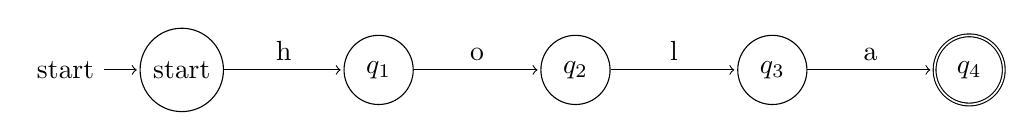
\begin{tikzpicture}[
        shorten >=1pt,
        node distance=2.5cm,
        on grid,
        auto
    ]
        \node[state, initial] (q0) {start};
        \node[state] (q1) [right=of q0] {$q_1$};
        \node[state] (q2) [right=of q1] {$q_2$};
        \node[state] (q3) [right=of q2] {$q_3$};
        \node[state, accepting] (q4) [right=of q3] {$q_4$};

        \path[->]
        (q0) edge node {h} (q1)
        (q1) edge node {o} (q2)
        (q2) edge node {l} (q3)
        (q3) edge node {a} (q4);
    \end{tikzpicture}
    \caption{Transiciones para la frase "hola" tipo SALUDO}
\end{figure}


El \textbf{AFD} (Autómata Finito Determinista) implementado en este proyecto tiene como
objetivo reconocer frases o palabras clave dentro de un texto, asignando un \textit{token} con
tipo semántico (saludo, despedida, etc.) y puntuación según una tabla predefinida. Este
autómata no está construido manualmente, sino que se genera dinámicamente a partir de listas de
palabras/frases, agrupadas por tipo.

\subsubsection{Construcción del AFD}

Para cada palabra o frase $\omega = c_1 c_2 \ldots c_n$ asociada a un tipo $T$:
\begin{enumerate}
	\item Se comienza desde el estado inicial $q_0$.
	\item Por cada caracter $c_i$ se crea un estado nuevo (si no existe) y una transición desde el estado actual.
	\item El último estado creado $q_n$ se marca como \textit{final}, y se le asigna el tipo de token $T$ y el puntaje de la frase.
\end{enumerate}

Así, frases distintas que comparten prefijos (por ejemplo, \texttt{"buen"} y \texttt{"buenos
	días"}) comparten transiciones, optimizando el tamaño del autómata.

Una vez construido, el AFD se guarda como un archivo \texttt{afd.json}, permitiendo depuración
y visualización externa.

\subsubsection{Reconocimiento de tokens}

Para tokenizar un texto:
\begin{enumerate}
	\item Se itera carácter por carácter desde la posición actual $i$ del texto.
	\item Se mantienen múltiples rutas activas en paralelo (cada una con estado actual, acumulador de caracteres y longitud).
	\item Cuando una ruta alcanza un estado final, se guarda como el mejor token candidato hasta el momento.
	\item Si se encuentra un token más largo, se reemplaza el candidato anterior.
	\item Al terminar el recorrido, si se detectó un token válido, se retorna. Si no, se interpreta como una palabra genérica.
\end{enumerate}

\subsubsection{Características adicionales}

\begin{itemize}
	\item El autómata diferencia hablantes mediante tokens como \texttt{agente:} o \texttt{cliente:}.
	\item Se identifican signos de puntuación como tokens individuales.
	\item Si una palabra no es reconocida por el AFD, se busca en la tabla de sentimientos como palabra suelta.
\end{itemize}

\subsection{Estructura de Datos}
El AFD tiene un diccionario para almacenar las transiciones entre estados y otro para los
identificadores de lexemas. Un contador permite llevar el registro de cuántas veces se han
reconocido las palabras de cada categoría. La tabla de sentimientos utiliza una lista enlazada
donde es posible agregar o eliminar palabras y ponderaciones mediante el menú del sistema.




\subsection{Análisis de Sentimiento}
Se utiliza una tabla de sentimientos que asigna puntajes a palabras positivas y negativas. Al
procesar los lexemas, se acumula un puntaje total que determina si el sentimiento general de la
interacción es positivo, negativo o neutral.

\subsection{Verificación del Protocolo de Atención}
Se verifica si se cumplen ciertas condiciones de atención al cliente, como la presencia de
saludos y despedidas, y se detectan palabras que no son apropiadas.

\subsubsection{Salida de Resultados}
Los resultados del análisis, que incluyen el sentimiento general, puntajes, palabras
clasificadas, y la verificación del protocolo, se guardan en un archivo de texto y en un
archivo JSON que representa el estado del AFD.

\subsection{Decisiones Tomadas}

\subsubsection{Selección de un AFD}

\subsubsection{Definición de Estados y Transiciones}
Se definieron múltiples estados finales en el AFD, cada uno asociado a distintas categorías de
palabras: saludos, identificaciones, despedidas, palabras prohibidas, palabras positivas y
palabras negativas. Esta organización estructurada permite un análisis claro y eficiente de las
interacciones con los clientes. Las palabras correspondientes a cada categoría se cargan
previamente desde archivos de texto, listos para su uso en el análisis.

Las transiciones del autómata se implementaron para reconocer un conjunto específico de
palabras, seleccionadas cuidadosamente para representar las categorías relevantes dentro del
contexto de atención al cliente y la verificación del protocolo que debe seguir el agente en
diversas situaciones.

\subsubsection{Implementación de la Tokenización}
Se optó por utilizar expresiones regulares para extraer lexemas del texto de entrada. Este
enfoque permite una identificación precisa de las palabras individuales y su procesamiento en
el AFD. Se incorporó un manejo de errores léxicos mediante la creación de un estado
\textbf{q\_ERROR\_LX} para capturar palabras no reconocidas. Esto mejora la robustez del
algoritmo al permitir una respuesta adecuada ante entradas inesperadas.

\subsubsection{Verificación del Protocolo}
Se implementó un mecanismo para verificar el cumplimiento del protocolo de atención al cliente,
asegurando que las interacciones contengan elementos clave como saludos y despedidas. Esto
ayuda a evaluar la calidad del servicio proporcionado por el agente. Esta decisión se tomó con
el objetivo de garantizar que el análisis no solo sea técnico, sino también relevante para las
prácticas de atención al cliente.

\subsubsection{Salida y Visualización de Resultados}
Se decidió que los resultados del análisis se guardarían tanto en un archivo de texto como en
un archivo JSON. Esto permite no solo una fácil revisión por parte de los usuarios, sino
también la posibilidad de almacenar el estado del AFD para futuros análisis. La estructura JSON
se eligió para facilitar la visualización y el análisis posterior del comportamiento del AFD y
el funcionamiento de las transiciones.

%%%%%%%%%%%%%%%%%%%%%%%%%%%%%%%%%%%%%%%%%%%%%%%%%%%%%%
%                Alcance guau                        %
%%%%%%%%%%%%%%%%%%%%%%%%%%%%%%%%%%%%%%%%%%%%%%%%%%%%%%
\subsection{Alcance del Proyecto}
El alcance del proyecto se puede definir a través de los siguientes puntos clave:

\subsubsection{Clasificación de Lexemas}
El sistema identifica y clasifica lexemas en diferentes categorías, permitiendo una mejor
comprensión del contexto de la interacción. Esto incluye clasificaciones específicas para
saludos, identificaciones, despedidas, palabras prohibidas y palabras que expresan
sentimientos.

\subsubsection{Análisis de Sentimientos}
Se realiza un análisis de sentimientos sobre las interacciones, evaluando las palabras
utilizadas para determinar si la conversación fue positiva, negativa o neutral. Esto se realiza
mediante la tabla de sentimientos donde cada palabra posee una ponderación pre-cargada desde un
archivo de texto.

\subsubsection{Verificación de Protocolos de Atención}
El sistema verifica si se cumplen los protocolos de atención al cliente, asegurando que las
interacciones incluyan los elementos necesarios para una atención efectiva. Esto incluye la
detección de saludos y despedidas apropiadas por parte del agente.

\subsubsection{Manejo de palabras no clasificadas}
La implementación del estado q\_ERROR\_LX permite manejar palabras no reconocidas o errores
léxicos, mejorando la robustez del sistema ante entradas inesperadas.

\subsubsection{Generación de Informes}
Los resultados del análisis se generan en archivos de texto donde se imprimen los reportes, una
tabla de lexemas y un JSON con las transiciones de cada palabra analizada, lo que permite una
fácil revisión.

\subsection{Estrategias Aplicadas}
Las estrategias aplicadas en el desarrollo del sistema incluyen:

\subsubsection{Desarrollo Modular}
El sistema se construyó de manera modular, separando las diferentes funcionalidades en clases y
métodos. Esto permite un mantenimiento más sencillo y la posibilidad de añadir nuevas
características en el futuro.

\subsubsection{Uso de AFD para Eficiencia}
La elección de un AFD como base del sistema permite una evaluación rápida y eficiente de los
lexemas, facilitando el procesamiento de grandes volúmenes de texto de interacciones.

\subsubsection{Implementación de Tablas de Sentimientos}
Se diseñó una tabla de sentimientos que asigna puntajes específicos a palabras según su
connotación, lo cual permite un análisis más detallado y preciso de las emociones expresadas en
las interacciones. Estos datos, pre-cargados desde un archivo de texto para garantizar su
persistencia, incluyen la flexibilidad de agregar o eliminar palabras según se requiera,
facilitando así la personalización y actualización continua del análisis de sentimiento.

\subsubsection{Recopilación de Datos y Mejora Continua}
Se incorporó un enfoque que permite la adición de nuevas palabras a las categorías existentes,
lo que permite que el sistema evolucione a medida que se identifican nuevas necesidades esto
mediante el uso de documentos de texto donde las palabras son guardadas.

\subsubsection{Validación de Resultados}
Se implementaron mecanismos para validar los resultados del sistema, asegurando que los
análisis sean precisos y útiles para evaluar la calidad del servicio de atención al cliente.

\newpage
%%%%%%%%%%%%%%%%%%%%%%%%%%%%%%%%%%%%%%%%%%%%%%%%%%%%%%
%                codigo fuente                       %
%%%%%%%%%%%%%%%%%%%%%%%%%%%%%%%%%%%%%%%%%%%%%%%%%%%%%%
% NOTE: ver para borrar la verdad

\subsection{Código Fuente}
En esta sección, se presenta el código fuente del sistema desarrollado para el análisis de
interacciones en contact centers. El código está organizado en módulos, clases y métodos que
permiten la tokenización de texto, el análisis de sentimientos y la verificación de protocolos
de atención.

El sistema está estructurado de la siguiente manera:
\begin{tcolorbox}[colback=gray!10, colframe=gray!80, sharp corners, boxrule=0.5pt]
	\begin{verbatim}
    +-- audios
    |   +-- audio-texto.py
    |   +-- prueba-texto1-negativo.m4a
    |   +-- prueba-texto2-positivo.m4a
    +-- data
    |   +-- despedidas.txt
    |   +-- identificaciones.txt
    |   +-- palabras_prohibidas.txt
    |   +-- palabras_y_puntajes.txt
    |   +-- saludos.txt
    |
    +-- doc
    |   +-- ensayo.pdf
    |
    +-- models
    |   +-- afd.py
    |   +-- analisis.py
    |   +-- file_utils.py
    |   +-- menu.py
    |   +-- sentimientos.py
    |   +-- __init__.py
    |
    +-- output
    |   +-- afd.json
    |   +-- reporte.txt
    |   +-- tabla_lexemas.txt
    |
    +-- test
    |    +-- prueba-texto1-negativo.txt
    |    +-- prueba-texto2-positivo.txt
    |    +-- prueba-texto3-positivo.txt
    |    +-- prueba-texto4-neutral.txt
    |    +-- prueba.txt
    |
    |- tokenizador.py
    |- README.md

\end{verbatim}
\end{tcolorbox}
\newpage

% TODO: agregar una descripcion de las clases principales

\section*{Explicación de la Clase AFD}
\begin{quote}
	\textbf{Inicialización:} La clase \texttt{AFD} se inicializa definiendo el estado inicial, los estados finales y las transiciones que definen el flujo del autómata.\\
	\textbf{Métodos:}
	\begin{itemize}
		\item \textbf{agregar\_transicion:} Permite agregar transiciones entre estados mediante lexemas, asegurando que no haya duplicados en las transiciones.
		\item \textbf{evaluar\_lexema:} Evalúa si un lexema puede ser procesado desde el estado inicial hacia uno de los estados finales, indicando si se encontró una transición válida.
		\item \textbf{vaciar:} Reinicia el AFD, eliminando todas las transiciones y reiniciando los IDs de lexemas.
		\item \textbf{guardar\_en\_json:} Guarda el estado y las transiciones del autómata en un archivo JSON.
		\item \textbf{generar\_tabla\_lexemas:} Genera una tabla organizada de lexemas, mostrando su token y patrón asociado, para facilitar el análisis de la clasificación de palabras.
	\end{itemize}
\end{quote}


\section*{Estructura de la Tabla de Sentimientos}

La estructura de la \texttt{TablaSentimientos} y la clase \texttt{NodoSentimiento} permiten
almacenar y gestionar palabras asociadas a un puntaje de sentimiento en una lista enlazada.
Esta estructura se utiliza para calcular el puntaje de sentimiento de un conjunto de palabras.

\subsection*{Clase \texttt{NodoSentimiento}}
La clase \texttt{NodoSentimiento} representa un nodo en la lista enlazada y contiene los atributos:
\begin{itemize}
	\item \texttt{palabra}: La palabra asociada al sentimiento.
	\item \texttt{puntaje}: El puntaje de sentimiento de la palabra, que puede ser positivo, negativo o cero.
	\item \texttt{siguiente}: Referencia al siguiente nodo en la lista enlazada.
\end{itemize}

\subsection*{Uso de la Tabla de Sentimientos}
Esta estructura permite almacenar y recuperar palabras con sus puntajes de manera eficiente,
facilitando el análisis de sentimientos en otras funciones del programa mediante métodos de
inserción, búsqueda y eliminación en una lista enlazada.

\subsubsection{Gestión de Sentimientos}

\section*{Módulo de Gestión de Sentimientos}

Este módulo permite la carga, adición y eliminación de palabras con sus puntajes de sentimiento
en una \texttt{TablaSentimientos}, así como la actualización de un Autómata Finito Determinista
(AFD) para clasificar palabras. También se realiza la persistencia de datos en archivos.

\subsection*{Funciones Principales}

Este código implementa el flujo principal de un sistema de análisis de sentimientos y
verificación de protocolo de atención utilizando un AFD (Autómata Finito Determinista) y una
tabla de sentimientos.

\subsection*{Notas Importantes}
El código maneja los resultados de análisis de sentimientos y verificación de protocolo tanto
en la consola como en archivos de texto para su revisión.

\subsection{Resultados}
El siguiente es el resultado del análisis de un ejemplo de conversación entre un agente y un
cliente, en el cual se detecta un sentimiento general positivo. Los tokens asociados a palabras
positivas superan en número y en puntaje a las palabras negativas, lo que sugiere una
interacción satisfactoria. Además, se verifica que el agente ha cumplido con el protocolo de
atención al cliente, incluyendo saludo, identificación, y despedida, sin utilizar palabras
prohibidas.

\subsection*{Link del Repositorio:}
\href{https://github.com/AlexArce2000/tokenizador-tp-compiladores}{Repositorio Github}

\subsection*{Caso de ejemplo}
\subsection*{Entrada:}
\begin{verbatim}
-----------------------------------------------------------------    
Agente: ¡Buenos días! Gracias por contactar con el servicio al 
cliente de ConexiónNet. Mi nombre es Johanna. ¿Cómo puedo 
ayudarle hoy?

Cliente: Hola, estoy teniendo algunos problemas con mi 
internet. Pago por 100 Mbps, pero últimamente he notado que 
la velocidad es mucho más baja.

Agente: Lamento escuchar eso, y estoy aquí para ayudarle 
a resolverlo. ¿Podría proporcionarme su nombre completo 
y el número de cuenta para que pueda revisar su situación?

Cliente: Claro, soy Juan Pérez y mi número de cuenta es 
12345678.

Agente: ¡Gracias, Juan! Voy a revisar su cuenta ahora mismo.
Veo que efectivamente tiene un plan de 100 Mbps. 
Déjeme hacer una prueba de línea para verificar cómo está 
funcionando su conexión en este momento.

Cliente: Sí, por favor. Me gustaría que se resolviera pronto.

Agente: ¡Entiendo perfectamente! Estoy realizando la prueba.
Vaya, parece que hay algunas fluctuaciones en la señal. 
No se preocupe, eso es algo que podemos solucionar. Voy a 
reiniciar su línea desde aquí, lo que puede ayudar a estabilizar 
la conexión. Esto tomará solo un minuto, y perderá la conexión 
brevemente. ¿Le parece bien?

Cliente: Sí, eso suena bien. Espero que funcione.

Agente: ¡Genial! Estoy reiniciando su línea. Listo. 
El reinicio se ha completado. Ahora, por favor, reinicie también 
su módem y router manualmente. Simplemente desconéctelos de la 
corriente durante 30 segundos y luego vuelva a conectarlos. Esto 
debería refrescar la señal.

Cliente: Está bien, lo haré. ¿Y si eso no soluciona el problema?

Agente: Si después de reiniciar su equipo el problema persiste, 
no se preocupe. Programaremos una visita de un técnico a su 
domicilio para asegurarnos de que todo esté en orden. Queremos 
que disfrute del servicio por el que está pagando.

Cliente: Eso suena bien. Solo quiero que funcione como debería.

Agente: Lo comprendo completamente, Juan. Estoy segura de que 
podremos resolver esto. Espero que el reinicio funcione, pero 
si no, estaremos aquí para ayudarle. ¿Hay algo más en lo que 
pueda asistirte hoy?

Cliente: No, eso es todo. Solo espero que se solucione pronto.

Agente: ¡Perfecto! Agradezco su paciencia y confianza. No dude 
en llamarnos si necesita algo más. Le deseo un excelente día 
y que su servicio se estabilice pronto. 
¡Estamos aquí para ayudarle!

Cliente: Gracias, adiós.

Agente: ¡Adiós, Juan! Que tenga un buen día.
----------------------------------------------------------------- 
\end{verbatim}

\subsection*{Salida:}
\begin{tcolorbox}[colback=gray!10, colframe=gray!80, sharp corners, boxrule=0.5pt]
	\begin{verbatim}
Sentimiento general: Positivo
Puntaje total: 12
Palabras positivas: ['bien', 'bien', 'genial', 'bien', 'bien', 
'perfecto', 'paciencia', 'excelente']
Palabras negativas: ['problema', 'problema']
Verificación del protocolo de Atención (Agente):
    - Saludo: OK
    - Identificación: OK
    - Despedida: OK
    - Palabras rudas: Ninguna detectada
\end{verbatim}
\end{tcolorbox}

\section{Conclusión}

Este proyecto implementa un sistema integral de análisis de sentimientos y verificación de
protocolos de atención mediante el uso de un Autómata Finito Determinista (AFD) y una tabla de
sentimientos. La arquitectura del sistema permite la identificación y clasificación de palabras
con carga emocional, así como la detección de palabras inapropiadas en las interacciones.
Además, el sistema verifica el cumplimiento de los elementos fundamentales del protocolo de
atención (saludo, identificación y despedida), proporcionando una evaluación detallada de las
respuestas del agente.

La flexibilidad del sistema para agregar o eliminar palabras de la tabla de sentimientos y
actualizar el AFD en tiempo real lo hace adaptable a nuevas necesidades o criterios específicos
de análisis. Esta capacidad de modificación y persistencia de datos asegura que el sistema se
pueda ajustar continuamente para mejorar la precisión de las evaluaciones y adaptarse a
diferentes contextos de uso.

En conjunto, este sistema representa una herramienta robusta y adaptable para el análisis
automatizado de interacciones en centros de contacto, con potencial de ser extendido o
integrado en aplicaciones más amplias de procesamiento de lenguaje natural (PLN) o de mejora de
calidad en la atención al cliente.

\end{document}
